\documentclass{article}
%\usepackage[spanish]{babel} 
%\selectlanguage{english}  
\usepackage[utf8]{inputenc} 
\usepackage[T1]{fontenc} 
\usepackage{array}
\usepackage{geometry}
 \geometry{
 a4paper,
 total={170mm,257mm},
 left=20mm,
 top=20mm,
 }
\usepackage{amsmath, amsthm, amsfonts} 
\usepackage{graphicx} 
\usepackage[colorinlistoftodos]{todonotes} 
\usepackage[colorlinks=true, allcolors=blue]{hyperref} 
\usepackage[square,numbers]{natbib}
\usepackage{upgreek}
\usepackage{lipsum}  
\usepackage{diagbox}


\title{Informe del Proyecto Final Grupo 6}
\author{Benjam\'in Ignacio Ayala Baeza  \\ \href{mailto:beayala2021@udec.cl}{beayala2021@udec.cl} 
        \and Mar\'ia Ignacia Espinoza Inzunza \\ \href{mailto:marespinoza2021@udec.cl}{marespinoza2021@udec.cl} \\
        \and Florencia Andrea Fuentes Jara \\ \href{mailto:flofuentes2021@udec.cl}{flofuentes2021@udec.cl} \\
        \and Mart\'in Andrés Sepúlveda Zu\~niga \\ \href{mailto:msepulveda2021@udec.cl}{msepulveda2021@udec.cl} \\
\date{Universidad de Concepci\'on \\ \today}
}
\setlength{\marginparwidth}{2cm}

%-------------------------------------------------------------------------------------------------------------------------

\begin{document}

\maketitle

\begin{abstract}
En el presente documento buscamos encontrar la relación entre la distancia de lanzamiento de una fuerza aplicada a un cuerpo circular y el giro que se produce. Esto midiendo el número de giros a distintas distancias del cuerpo y con varias repeticiones para eliminar el error aleatorio. Además graficamos nuestros datos y realizamos varios ajustes para analizar cuál se asimila más a nuestro modelo esto viéndolo con el análisis de sus respectivos residuos y así concluir con alguna correspondencia entre nuestras variables.
\end{abstract}

\section{Introducción} \label{intro}
 En este informe decidimos realizar un proyecto que surgió bajo el interés de saber cuanto rota una cinta métrica al lanzar la espiga a distintas distancias de la cinta, en términos físicos, nuestra premisa para este experimento consta de estudiar de una manera eficaz los efectos de una fuerza aplicada de manera tangencial a un objeto que posee una capacidad de rotación.
 \medskip
 Primero, definiremos algunos conocimientos previos necesarios para poder eventualmente comparar el comportamiento de los datos con los fenómenos físicos, luego ilustraremos los procedimientos necesarios que realizaremos en la etapa de experimentación, además de los resultados obtenidos en esta y poder así realizar ajustes con distintos modelos con el fin de analizar si estos se asimilan a el comportamiento natural de estos datos a través del análisis de sus residuos. Finalmente concluiremos explicando cual modelo se ajusta mejor a los datos y como este comportamiento corresponde a lo esperado por las leyes de la física. 

\section{Objetivos}
Nuestros objetivos a lograr con esta actividad de laboratorio son :

\begin{itemize}
    \item Encontrar la relación entre la distancia de lanzamiento del medidor de una cinta métrica con el número de giros que esta hace en una plataforma en nuestro caso la mesa del laboratorio.
    \item Comparar nuestros resultados con algún hecho cotidiano o fenómeno físico relacionado.
\end{itemize}

\section{Marco Teórico}
Para el desarrollo de este informe haremos uso de las siguientes ecuaciones y términos físicos:

\begin{itemize}
    \item \textbf{Ángulo de rotación:} Medida del giro de una figura alrededor de un punto fijo.
    \item \textbf{Fuerza:} Acción, esfuerzo o influencia que puede alterar el estado de movimiento o de reposo de cualquier cuerpo. El cual se puede medir con la siguiente formula dada por la segunda ley de newton :
    \begin{equation*}
       \vec F = m \cdot \vec a
    \end{equation*}
    \item \textbf{Aceleración Tangencial:}
    \item \textbf{Fuerza Tangencial:}
\end{itemize}

\section{Experimentación}
Para encontrar la correlación entre distancia y cantidad de vueltas del cuerpo de la cinta de medir, debemos repetir el experimento en diversas condiciones. Nuestra condición variable corresponde a la distancia desde la cual veremos como afecta la fuerza de choque tangencial de la espiga con el cuerpo de esta.

\subsection{Materiales}
En este proyecto utilizamos los siguientes instrumentos:
\begin{itemize}
    \item[-] Cinta Métrica 3$[\text{m}]$
    \item[-] Papel con ejes de referencia
    \item[-] Cinta adhesiva
    \item[-] Celular con cámara lenta
    \item[-] Mesa
\end{itemize}
    
\subsection{Montaje Experimental}
  En la figura \ref{fig:montaje} mostramos los materiales utilizados para el montaje de nuestro experimento.
  
\begin{figure}[ht]
    \centering
    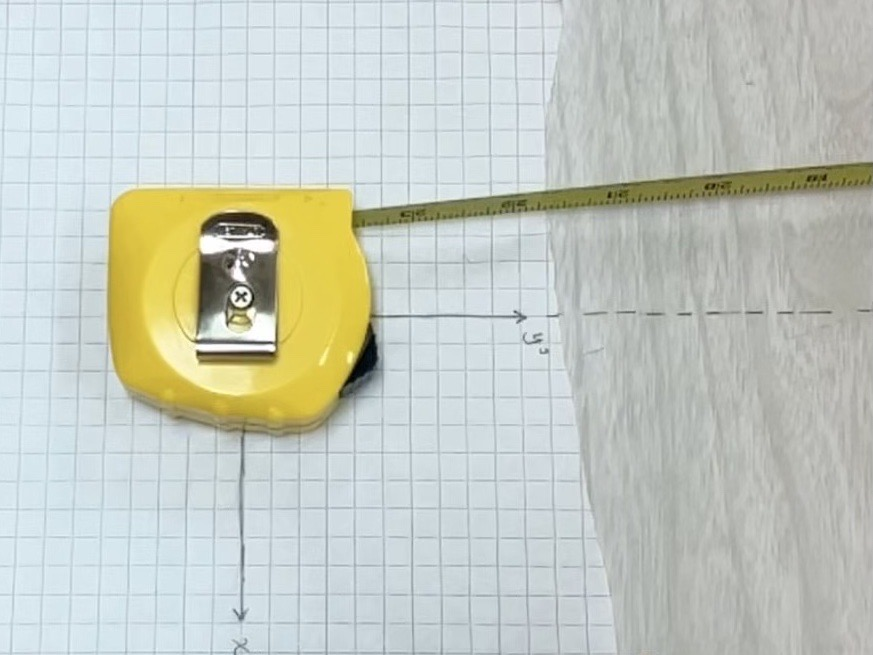
\includegraphics[scale=0.25]{Informe/img/montaje1.png}
    \caption{Fotografía de montaje experimental}
    \label{fig:montaje}
\end{figure}
    
\subsection{Procedimiento}
A continuación describiremos detalladamente el paso a paso realizado para las diversas mediciones hechas:

\begin{enumerate}
    \item Comenzamos colocando la cinta métrica al centro del papel con ejes de referencia, de forma que si extendemos la cinta métrica esta crece a lo largo del eje de las ordenadas. La cinta métrica y debe estar pegada al papel, esto lo logramos usando la cinta adhesiva.
    \item Alineamos en nuestra mesa el papel con ejes de referencia y proyectamos estos ejes en la mesa, de forma que tengamos una extensión de estos para observar cuanto gira el montaje de la cinta métrica con el papel. 
    \item Posicionamos nuestro celular con cámara lenta por encima del montaje del papel, mesa y cinta de forma que tengamos una visión área del sistema.
    \item Tomamos la espiga de la cinta métrica y la extendemos hasta llegar a los $10[\text{cm}]$, luego soltamos esta y vemos cuanto giro se produce. Todo este proceso se graba con el celular. \label{4} 
    \item Repetimos el paso \ref{4} diez veces. \footnote{Idealmente recomendamos tomar más repeticiones, ya que entre más repeticiones menos error aleatorio va a existir, sin embargo, para este proyecto en particular por temas de tiempo tuvimos que mantenernos en diez repeticiones.}
    \item Repetimos todo el procedimiento para la medida de la cinta métrica en incrementos de $10[\text{cm}]$, hasta llegar a los $100[\text{cm}]$.
\end{enumerate}

\subsection{Procesamiento de datos}
El procedimiento para la extracción de datos, en este caso el ángulo total de giro, se hizo mediante el análisis de imágenes que se extrajeron de los vídeos, considerando este ángulo de giro desde que la espiga de la cinta métrica choca con el cuerpo de esta, y hasta que este deja de girar. Para esto se utilizo un programa de edición de imágenes con el que contaba con una escuadra digital, la cual tenia una sensibilidad de $0.5^{\circ}$. 

\medskip
Se implementaron dos marcos de referencia en la imagen obtenida, uno se ubico en la superficie en la que se hizo el experimento, la cual se encontraba en reposo, y el segundo se ubico en la cinta métrica, la cual era un sistema dinámico. Luego se comparo el ángulo entre los estados iniciales de cada sistema y el estado final de cada sistema, así obteniendo el ángulo total de giro de la cinta, esto se repitió para cada iteración de longitud.

\section{Resultados y Análisis}
A continuación, expondremos nuestros datos recopilados durante las mediciones. Comenzaremos mostrando el gráfico que se puede ver en la figura \ref{fig:datos}, en donde nos muestra la cantidad de vueltas expuestas según la distancia tomada, donde el eje de las abscisas corresponde a la longitud desde la cual soltamos la cinta métrica y el eje ordenado la cantidad de grados que este ha rotado. Este gráfico fue construido a partir de los datos que pueden ser encontrados en \href{https://github.com/ayalin7/El-proyectito/blob/main/graficos/datos/giro.txt}{este link}. \\
A partir de esto podemos ver una clara tendencia al aumento de la cantidad de vueltas en función de la distancia desde la cual soltamos la cinta métrica lo cual hará sentido poniendo en comparativa la relación entre la segunda derivada de la longitud (correspondiente a la aceleración), la masa y la fuerza con la cual gira sobre si misma la cinta métrica. 

Para continuar con el análisis de este fenómeno, comenzamos con un trabajo computacional sobre los datos

% agregar lo de los diferentes ajutes y como hay una que tiene la mejor curva, en función del chi cuadrado que aumenta en consideración con los diversos coeficientes de las funciones del ajuste. 

\begin{table}[]
\centering
\begin{tabular}{|c|c|c|}
\hline
\small{Longitud del tiro} & Promedio[$\bar{x}$]  & Desviación Estándar [$\sigma$]\\ \hline
 10  \scriptsize{$[\text{cm}]$} & $63.6^\circ$  & $\pm 18.5^\circ$  \\ \hline
 20  \scriptsize{$[\text{cm}]$} & $193.8^\circ$ & $\pm 14.6^\circ$  \\ \hline
 30  \scriptsize{$[\text{cm}]$} & $266.1^\circ$ & $\pm 34.2^\circ$  \\ \hline
 40  \scriptsize{$[\text{cm}]$} & $370.8^\circ$ & $\pm 81.8^\circ$  \\ \hline
 50  \scriptsize{$[\text{cm}]$} & $439.3^\circ$ & $\pm 89.0^\circ$  \\ \hline
 60  \scriptsize{$[\text{cm}]$} & $495.5^\circ$ & $\pm 79.9^\circ$  \\ \hline
 70  \scriptsize{$[\text{cm}]$} & $508.9^\circ$ & $\pm 76.5^\circ$  \\ \hline
 80  \scriptsize{$[\text{cm}]$} & $621.3^\circ$ & $\pm 97.8^\circ$  \\ \hline
 90  \scriptsize{$[\text{cm}]$} & $621.6^\circ$ & $\pm 97.4^\circ$  \\ \hline
 100 \scriptsize{$[\text{cm}]$} & $682.8^\circ$ & $\pm 75.5^\circ$  \\ \hline 
\end{tabular}
\caption{Promedio y desviación estándar de las iteraciones mediadas en cada longitud de tiro}
\end{table}

\begin{figure}[ht]
    \centering
    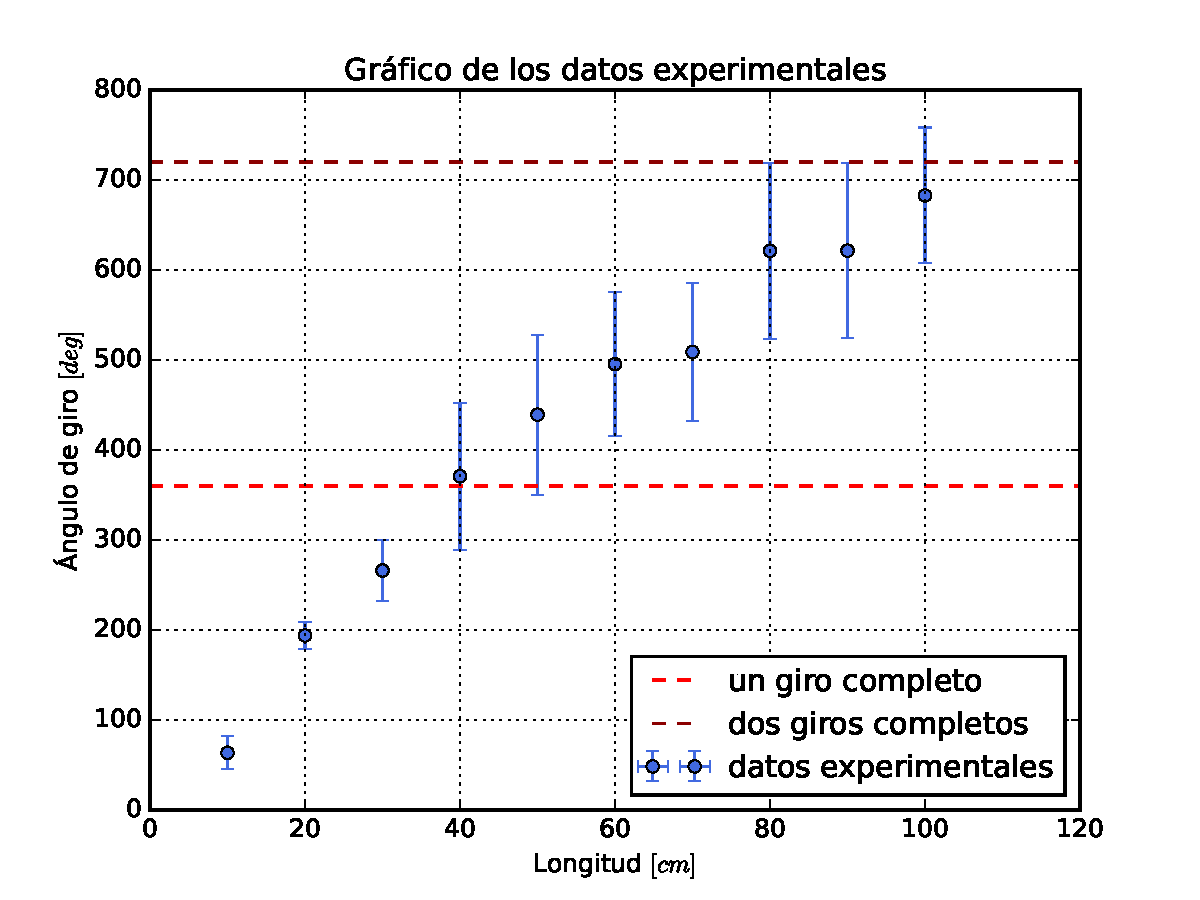
\includegraphics[scale=0.5]{Informe/img/grafico-datos.pdf}
    \caption{Gráfico formado a partir de los datos recopilados. El código de este gráfico se encuentra haciendo clic \href{https://github.com/ayalin7/El-proyectito/blob/main/graficos/grafico-datos.py}{aquí}.}
    \label{fig:datos}
\end{figure}

\begin{figure}[ht]
    \centering
    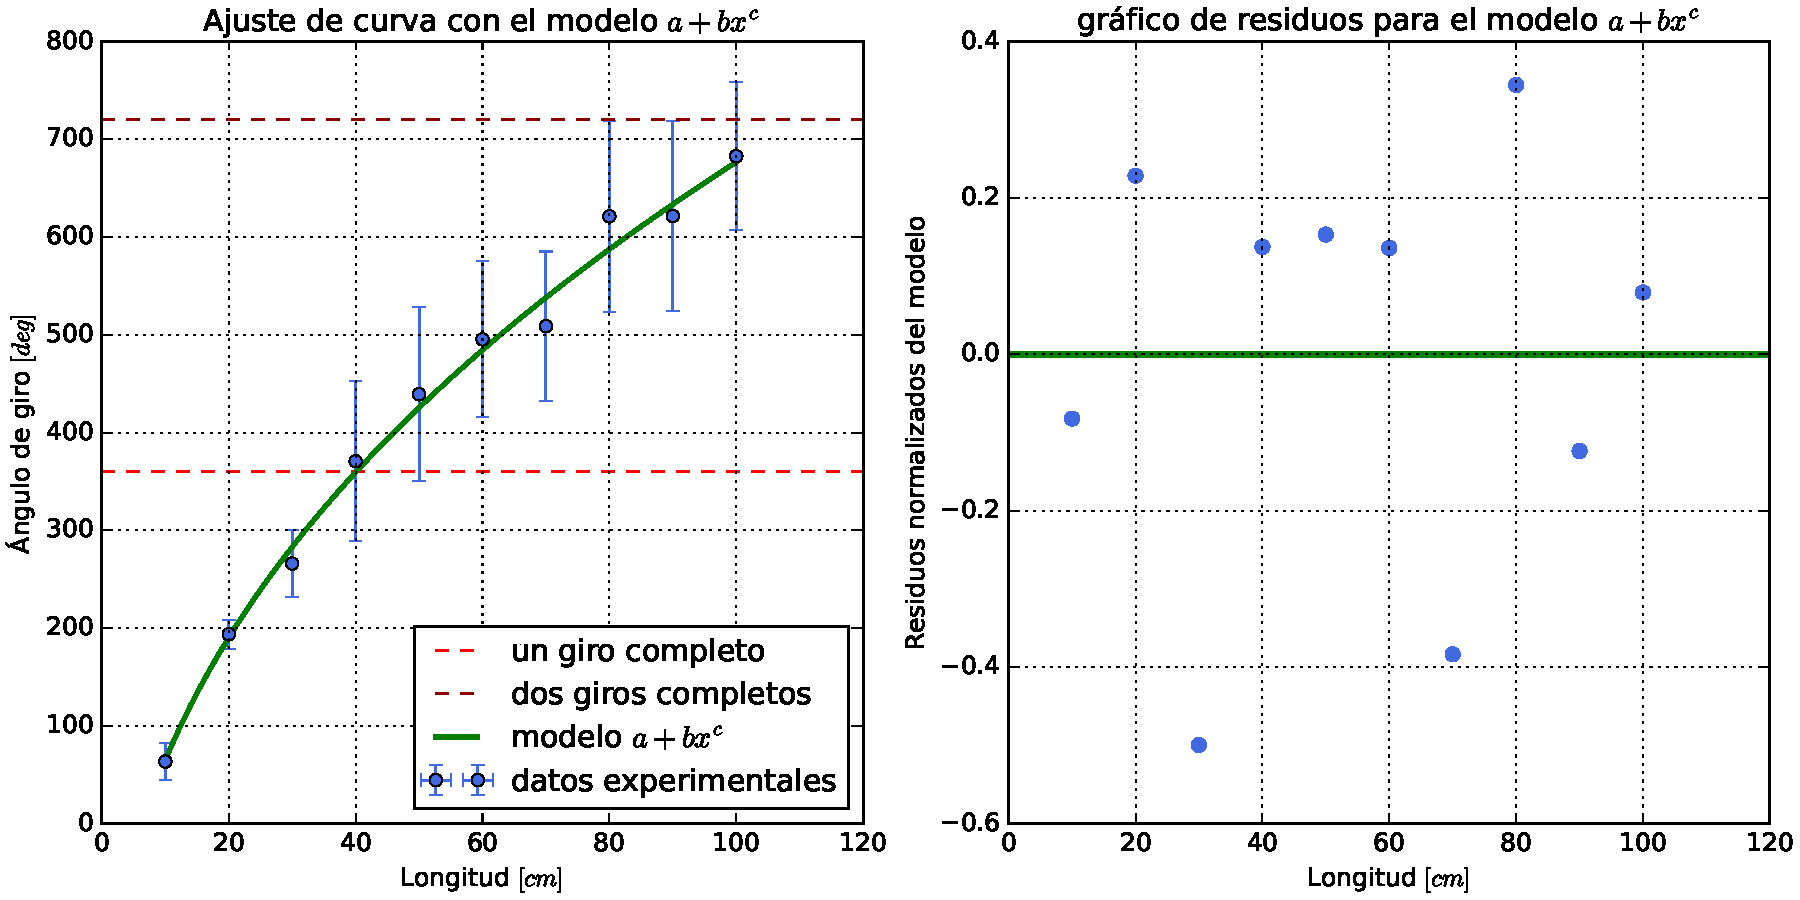
\includegraphics[scale=0.5]{Informe/img/grafico-modelo-axb.pdf}
    \caption{gráfico del modelo $a + bx^{c}$, con su respectivo análisis de residuos, donde su $\chi^2 = 24.4$. El código de este gráfico se encuentra haciendo clic \href{https://github.com/ayalin7/El-proyectito/blob/main/graficos/grafico-modelo-axb.py}{aquí}.}
    \label{fig:axb}
\end{figure}

\begin{figure}[ht]
    \centering
    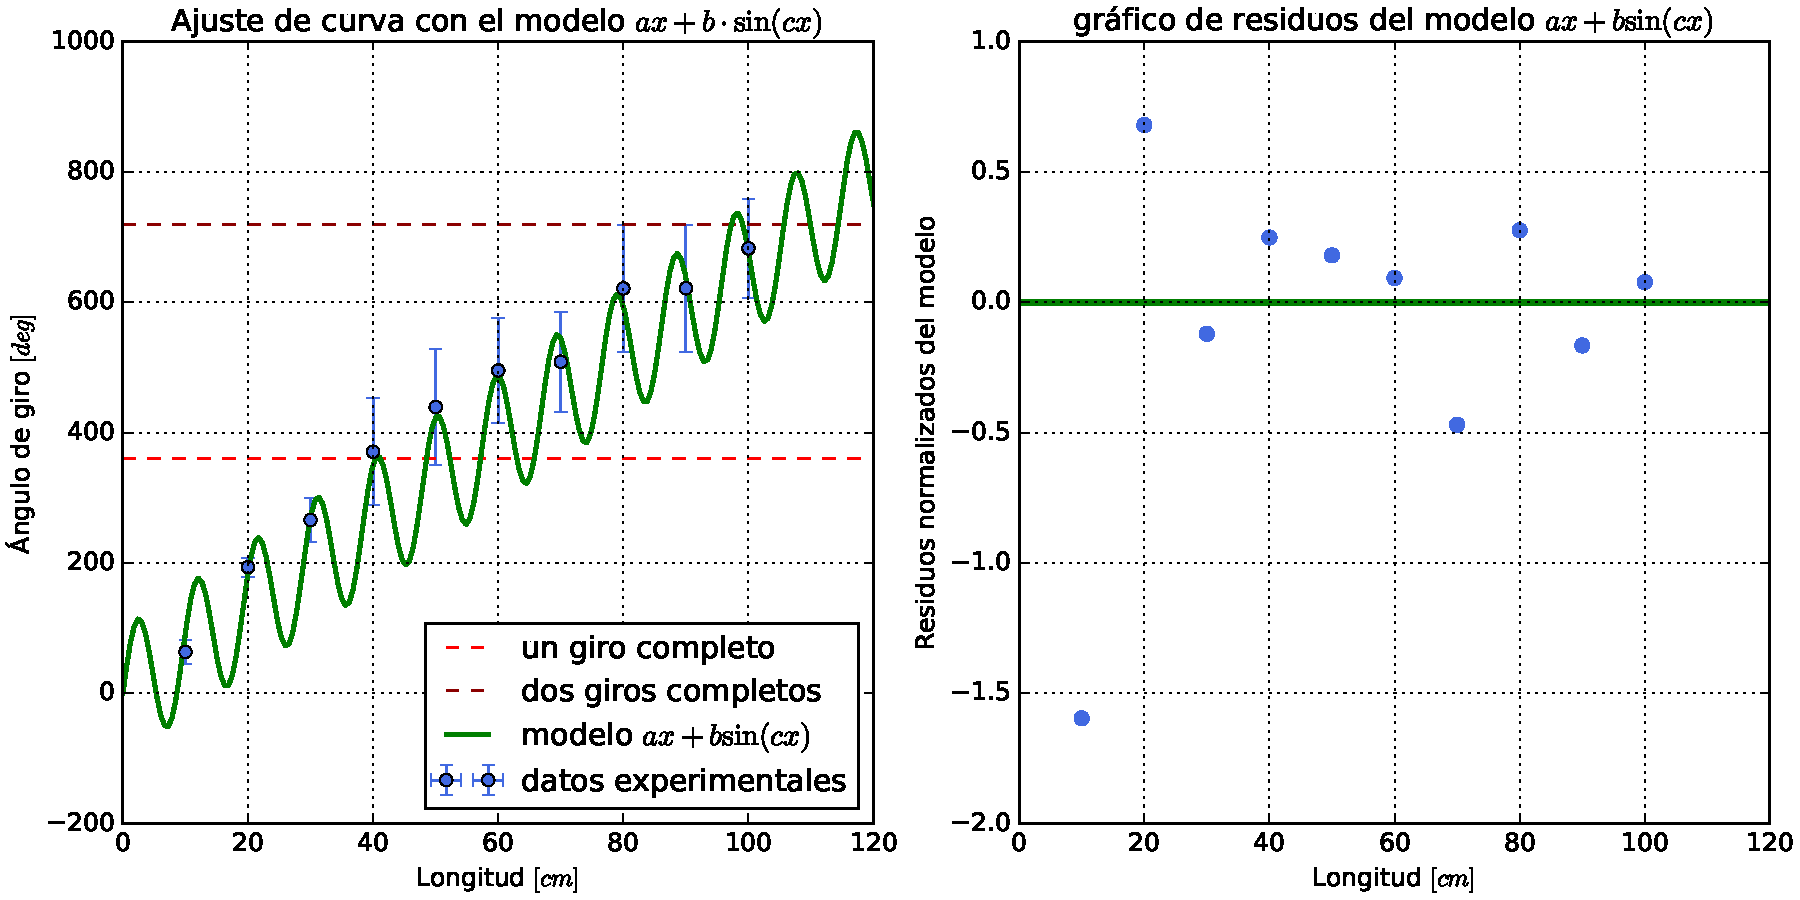
\includegraphics[scale=0.5]{Informe/img/grafico-modelo-asinb.pdf}
    \caption{gráfico del modelo $ax + b\sin(cx)$, con su respectivo análisis de residuos, donde su $\chi^2 = 43.9$. El código de este gráfico se encuentra haciendo clic \href{https://github.com/ayalin7/El-proyectito/blob/main/graficos/grafico-modelo-asinb.py}{aquí}.}
    \label{fig:asinb}
\end{figure}

\begin{figure}[ht]
    \centering
    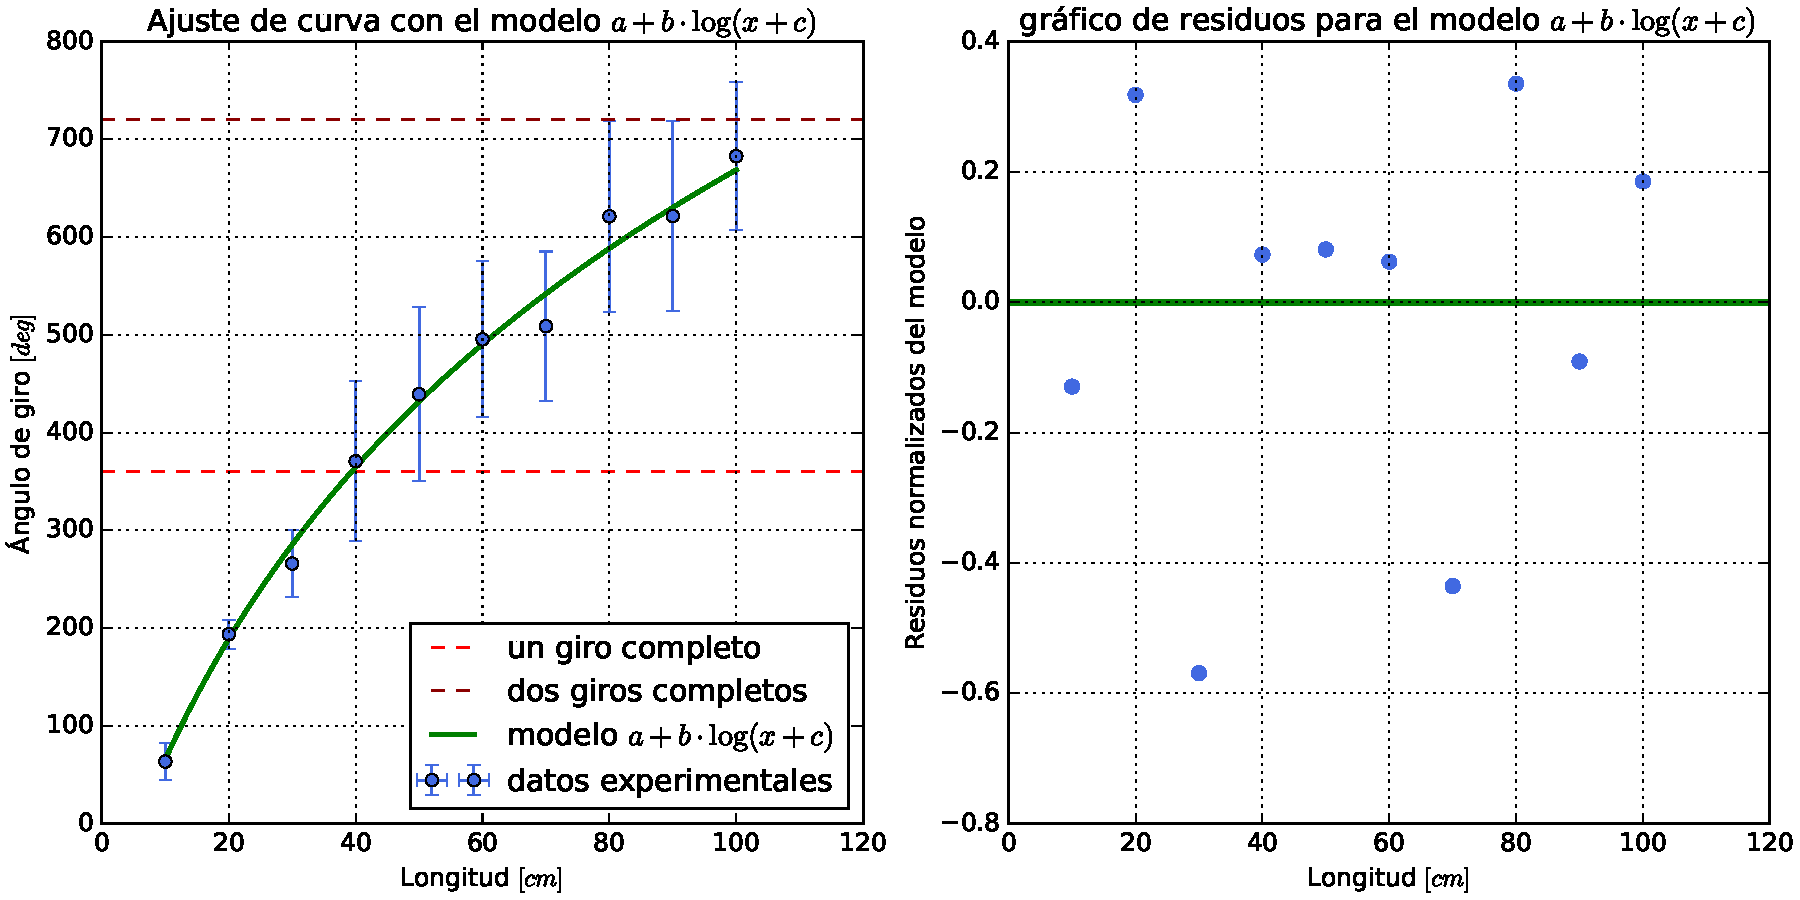
\includegraphics[scale=0.5]{Informe/img/grafico-modelo-alogb.pdf}
    \caption{gráfico del modelo $a + b \cdot \log(x + c)$, con su respectivo análisis de residuos, $\chi^2 = 21.1$. El código de este gráfico se encuentra haciendo clic \href{https://github.com/ayalin7/El-proyectito/blob/main/graficos/grafico-modelo-alogb.py}{aquí}.}
    \label{fig:alogb}
\end{figure}

\section{Conclusión}
Se concluye lo concluido por la conclusión que queda concluido lo que concluye finalmente.

\bibliographystyle{apalike}
\bibliography{Informe/referencias.bib}
\end{document}